\begin{fullwidth}
\chapter{Fisher Consistency of Ordinal Regression \mbox{Methods}}\label{chap:consistency}
\end{fullwidth}
\markright{{~{\rm \ref{chap:consistency}}. Fisher Consistency of Ordinal Regression Methods}\hfill}{}


\vspace*{\fill}

Ordinal regression is the supervised learning problem of learning a rule to predict labels from an ordinal scale. Ordinal regression models enjoy a wide applicability and some ordinal regression models have already been  used in Chapter 4 to model the decoding problem when the target variable consists of ordered values.


Many of the ordinal regression models that have been proposed in the literature can be viewed as methods that minimize a convex surrogate of the zero-one, absolute (as the methods presented in Chapter 4), or squared errors. In this chapter we investigate some theoretical properties of ordinal regression methods. The property that we will investigate is known as \emph{Fisher consistency} and relates the minimization of a given loss to the minimization of its surrogate. 


We provide a theoretical analysis of the Fisher consistency properties of a rich family of surrogate loss functions, including proportional odds and support vector ordinal regression. For all the surrogates considered, we either prove consistency or provide sufficient conditions under which these approaches are consistent. Finally, we illustrate our findings on real-world datasets.

\begin{shaded}
The contributions developed in this chapter are available in the submitted paper
\begin{itemize}
\item F. Pedregosa-Izquierdo, F. Bach, and A. Gramfort, \emph{``On the Consistency of Ordinal Regression Methods''}.
\end{itemize}
\end{shaded}

\vspace*{\fill}



\newpage 
\vspace*{\fill}
\minitoc
\vspace*{\fill}
\newpage


\section{Introduction}



In ordinal regression the goal is to learn a rule to predict labels from an ordinal scale, i.e., labels from a discrete but ordered set. This arises often when the target variable consists of human generated ratings. Besides the examples of ordinal labels in the context fMRI-based brain decoding presented in Chapter 4, examples of ordinal scales include (``do-not-bother'' $\prec$ ``only-if-you-must'' $\prec$ ``good'' $\prec$ ``very-good'' $\prec$ ``run-to-see'') in movie ratings~\citep{crammer2001pranking},  (``absent'' $\prec$ ``mild'' $\prec$ ``severe'') for the symptoms of a physical disease~\citep{ARMSTRONG01011989} and the NRS-11 numeric rating scale for clinical pain measurement~\citep{PAPR:PAPR3034}. Ordinal regression models have been successfully applied to fields  as diverse as econometrics~\citep{greene1997econometric}, epidemiology~\citep{ananth1997regression}, fMRI-based brain decoding~\citep{doyle2013multivariate} and collaborative filtering~\citep{Rennie}.

In this chapter we turn to study some theoretical properties of these methods. The aim is that a theoretical approach allows a better understanding the methods at hand. For example, \citet{Keerthi2003} proposed two different models for the task of ordinal regression: SVOR with explicit constraints and SVOR with implicit constraints. In that work, the second approach obtained better generalization error in terms of the absolute error loss function. Similar results were obtained by~\citep{lin2006large} replacing the hinge loss by an exponential loss. Yet again, \citep{Rennie} arrived to similar conclusions by considering the logistic loss instead. One of the motivations behind this chapter is to answer the question: is there a theoretical reason that can explain this behavior? By the end of the chapter we will give arguments to answer this and other relation questions.


Before introducing the general formulation of ordinal regression, we briefly recall the supervised learning setting described in Section~\ref{subsec:supervised_learning}. Let $(\XX, \mathcal{A})$ be a measurable space. Let $(X, Y)$ be two random variables with joint probability distribution $P$, where $X$ takes its values in $\XX$ and $Y$ is a random label taking values in a set of \emph{ordered categories} that we will denote $\mathcal{Y} = \{1, 2, \ldots, k\}$. In the ordinal regression problem, we are given a set of $n$ observations $\{(X_1,
Y_1), \ldots, (X_n, Y_n) \}$ drawn i.i.d.~from $X\times Y$ and a \emph{loss
function} $\ell: \mathcal{Y} \times \mathcal{Y} \rightarrow [0, \infty)$. The goal is to learn from the training examples a measurable mapping called a~\emph{classifier} $h: \XX \rightarrow \mathcal{Y}$ so that the \emph{risk} given below is as small as possible:
\begin{equation}
\label{eq:l_risk}
\mathcal{R}_{\ell}(h) = \EE_{X \times Y}(\ell(Y, h(X)))\quad.
\end{equation}


The setting above looks similar to that of a multiclass classification problem. However, a loss function used for multiclass classification such as the 0-1 loss is not sensitive to the distance among target values. On the other hand, in the ordinal regression setting, because of the order between labels, the loss function becomes lower as the distance among classes decreases. This has been formalized as the \emph{V-shape} property~\citep{Li2007}. We will say that a loss function is V-shaped if its forward difference, $\Delta\ell(i, j) = \ell(i, j+1) - \ell(i, j)$, verifies $\Delta\ell(i, j) \leq 0$ for $j \leq i$ and $\Delta\ell(i, j) \geq 0$ for $j > i$.

The \emph{absolute error} loss function ($\ell_{\mathcal{A}}(y, k) = |y-k|$) is an example of V-shaped loss function, although this property includes other loss functions, such as the \emph{squared error}, $\ell_{\mathcal{S}}(y, k) = (y-k)^2$ and the $0-1$ loss.

\begin{marginfigure}
\includegraphics[width=\linewidth]{chapter_4/v_shaped.pdf}
\caption{
     The absolute error, defined as $\ell(i, j) = |i - j|$, is a loss function that verifies the V-shape property. In the figure, a plot of the absolute error loss $\ell(i, j) = |i - j|$ with $j=3$.
}
\end{marginfigure}


Attempting to directly minimize Eq.~\eqref{eq:l_risk} is not feasible in practice for two reasons. First, the probability distribution $P$ is unknown and the risk must be minimized approximately based on the observations. Second, due to the non-convexity and discontinuity of $\ell$, the risk is difficult to optimize and can lead to an NP-hard problem~\citep{feldman2012agnostic,ben2003difficulty} (note that binary classification can be seen as a particular case of ordinal regression). It is therefore common to approximate $\ell$ by a function $\psi: \mathcal{Y} \times \RR^d \to \RR$, called a \emph{surrogate loss function}, which has better computational properties. Here $d$ is an integer that depends on the surrogate. For the methods that we consider $d$ will be equal to $1, k-1$ or $k$. The goal becomes to find the \emph{decision function} $f$ that minimizes instead the $\psi$-risk, defined as
\begin{equation}
\Rpsi(f) = \EE_{X \times Y}(\psi(Y, f(X))) \enspace.
\end{equation}

Fisher consistency is a desirable property for surrogate loss functions~\citep{Lin2004}. It implies that in the population setting, i.e., if the probability distribution $P$ were available, then optimization of the $\psi$-risk would yield a function (not necessarily unique) with smallest possible risk, known as \emph{Bayes predictor} and denoted by $h^*$. This implies that within the population setting, the minimization of the $\psi$-risk and the minimization of the risk both yield solutions with same risk. From a computational point of view, this implies that the minimization of the $\psi$-risk, which is usually a convex optimization problem and hence easier to solve than the minimization of the $\ell$-risk, does not penalize the quality of the obtained solution.


The chapter is organized as follows. In Section \ref{sec:problem_setting} we present the ordinal regression models that we will consider for study. These can be broadly separated into \emph{regression-based} and \emph{threshold-based}. Section \ref{sct:consistency} is divided into several parts. In the first part, we extend results from~\citet{Ramaswamy2012} and prove consistency of regression-based surrogates. Because of its practical interest, the rest of this section is devoted to investigate the consistency of threshold-based surrogates. Here we present our main results, which gives sufficient conditions under which these surrogates are consistent. We finish with experiments and conclusions.



\subsection{Related work}

Fisher consistency of binary and multiclass classification for the zero-one loss has been studied for a variety of surrogate loss functions (see~\cite{Bartlett2003,Tewari2007} and references therein). \citet{Ramaswamy2012} investigated the more general setting of multiclass classification with an arbitrary loss function, a setting that includes ordinal regression. The authors proved Fisher consistency of a surrogate loss function of the absolute error for the case of $k = 3$. However, this work did not prove consistency of this surrogate for $k > 3$, nor did it prove consistency for any squared error surrogate or for any of the threshold-based surrogates that represent the majority of traditional approaches for ordinal regression.


A related, yet different, notion of consistency is \emph{asymptotic consistency}. A surrogate loss is said to be asymptotically consistent if the minimization of the $\psi$-risk converges to the optimal risk as the number of samples tends to infinity. It has also been studied in the setting of supervised learning~\citep{stone1977consistent,Steinwart2002}. This chapter focuses solely on Fisher consistency, and for simplicity we will now use the term consistency to denote Fisher consistency.

{\bf Notation}. As in the previous chapter we will denote the sequence of numbers from one to $k$ as $[k] = \{1,~2, \ldots,~k \}$. Throughout this chapter we will use letter $k$ to denote the number of classes in the target space. 


\section{Ordinal regression models}\label{sec:problem_setting}

Different methods have been proposed to learn an ordinal regression model. The \emph{\mbox{regression-based} approach} treats the labels as real values. It uses a standard regression algorithm to learn a real-valued function, and then predicts by rounding to the closest label (see, e.g.,~\citet{kramer2001prediction} for a discussion of this method using regression trees). In this setting we will examine consistency of two different surrogate loss functions, the absolute error (that we will denote $\psi_{\mathcal{A}}$) and the squared error (denoted $\psi_{\mathcal{S}}$), which are convex surrogates of $\ell_{\mathcal{A}}$ and $\ell_{\mathcal{S}}$, respectively. Given $\alpha \in \RR$, $y \in [k]$, these are defined as
\begin{equation}\label{eq:regression_based_surrogates}
\psi_{\mathcal{A}}(y, \alpha) = |y - \alpha|, \quad \psi_{\mathcal{S}}(y, \alpha) = (y - \alpha)^2 \quad.
\end{equation}
Note that the loss functions $\ell_{\mathcal{A}}$ and $\ell_{\mathcal{S}}$ have the same expression as their surrogates, however the difference strives in that the surrogates are continuous functions in their second arguments while the loss functions take values in the discrete set $[k]$. The prediction function for these surrogates is given by rounding to the closest integer in $[k]$, i.e., $\text{pred}(\alpha) = \min_{i \in [k]} |i - \alpha|$. For half-integers, i.e., for number of the form integer + $\frac{1}{2}$, the rule is to round to the left, that is, $\text{pred}(1.5) = 1$, $\text{pred}(2.5) = 2$, etc.



While these approaches may lead to optimal predictors when no constraint is placed on the regressor function space as we will see in Section~\ref{subsec:regression-based}, in practice only simple function spaces are explored such as linear or polynomial functions. In these situations, the regression-based approach might lack flexibility. The \emph{\mbox{threshold-based} approaches}~\citep{McCullagh1980,Rennie,Keerthi2003,lin2006large} provides greater flexibility by seeking for both a mapping $f: \XX \to \RR$ and a non-decreasing vector $\btheta \in \RR^{k-1}$, often referred to as~\emph{thresholds}, that map the class labels into ordered real values. 

\begin{marginfigure}
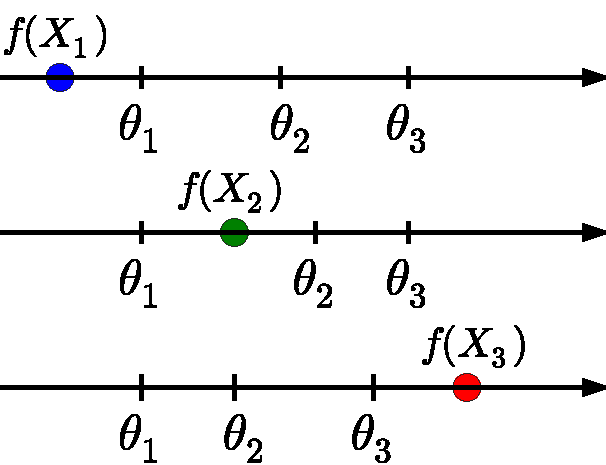
\includegraphics[width=\linewidth]{chapter_4/prediction.pdf}
\caption{In the ordinal logistic model, the thresholds partition the real line into $k$ segments and the prediction is given by the segment into which the decision function lies (assuming the segments are ordered by their relative order within the real line). Here, example for a 4-class problem. The prediction $f(X)$ for a given sample is denoted by a colored circle and $\theta_1, \theta_2, \theta_3$ are the estimated thresholds for that sample. Prediction in this example would be 1, 2, 4 respectively.}\label{fig:threshold_prediction}
\end{marginfigure}



The thresholds $\balpha$ partition the real line into $k$ segments, and the prediction is given by the segment into which the prediction $f(x)$ lies in (Fig~\ref{fig:threshold_prediction}). If we introduce the auxiliary variable $\alpha_i = \theta_i - f(x)$, an equivalent formulation of this prediction function is
\begin{equation}\label{eq:pred_threshold}
\text{pred}(\balpha) = 1 + \sum_{i=1}^{k-1} \mathcal{H}(-\alpha_i) \enspace,
\end{equation}
where we recall that $\mathcal{H}$ is the Heaviside function, defined as $\mathcal{H}(x) = 1$ if $x \geq 0$ and $0$ otherwise.



%{\blue Comment on the partial thresholds~\citep{citeulike:578341}}.


In the context of threshold-based functions we will consider two different families of surrogate loss functions. The first family of surrogate loss function that we will consider is the \emph{cumulative link} surrogates of~\citet{McCullagh1980}. In such models the posterior probability is modeled as $P(Y \leq i|X\!=\!x) = \sigma(g_i(x))$, where $\sigma$ is an appropriate link function. We will prove consistency for the case where $\sigma$ is the sigmoid function, i.e., $\sigma(t) = 1/(1 + \exp(-t))$. In this case it is known as the \emph{proportional odds} model or \emph{cumulative logit} model. For $x \in \XX, y \in [k]$ and $\alpha_i = g_i(x)$, the proportional odds surrogate (denoted $\psi_{\mathcal{C}}$) is defined as
\begin{equation}\label{eq:propodds}
\psi_{\mathcal{C}}(y, \balpha) = 
\begin{cases}
-\log(\sigma(\alpha_1)) &\text{ if } y = 1 \\
-\log(\sigma(\alpha_y) - \sigma(\alpha_{y-1})) &\text{ if } 1 < y < k \\
-\log(1 - \sigma(\alpha_{k-1})) &\text{ if } y = k.
\end{cases}
\end{equation}



The second family of surrogate loss functions that we will consider are the \emph{margin-based} surrogate loss functions of which the \emph{ordinal logistic} model introduced in Chapter 4 is a particular example. For appropriate real-valued functions $\phi: \RR \to \RR$ such as the hinge loss or exponential loss, this surrogate separate target values by the largest margins centered around the thresholds~\citep{lin2006large}. Given $x \in \XX, y \in [k]$ and $\balpha \in \RR^{k-1}$, the margin-based surrogate (denoted $\psi^{\ell}_{\mathcal{M}}$) is given by
\begin{gather*}
\label{eq:sum_of_loss}
\psi^{\ell}_{\mathcal{M}}(y, \balpha) =
\sum_{i = 1}^{y-1} \Delta \ell(y, i)\phi(\alpha_i) - \sum_{i=y}^{k-1}\Delta \ell(y, i)\phi(-\alpha_i) \enspace.
\end{gather*}
We recall that $\Delta\ell(y, i) = \ell(y,i+1) - \ell(y, i)$. Note that the V-shape property implies $\Delta\ell(y, i) \geq 0$ for the elements in the first term and $\Delta\ell(y, i) \leq 0$ for elements in the second term, thus this surrogate is convex in its second argument if $\phi$ is a convex function.


This formulation parametrizes several popular approaches to ordinal regression. For example, let $\phi$ be the hinge loss and $\ell$ the zero-one loss, then $\psi^{T}_{\ell}$ coincides with the Support Vector Ordinal Regression (``explicit constraints'' variant) of~\citep{Shashua, Chu2007}. If instead the mean absolute loss is considered, this approach coincides with the ``implicit constraints'' formulation of the same reference. For other values of $\phi$ and $\ell$ this loss includes the approaches proposed in~\citep{Shashua,Keerthi2003,Rennie,lin2006large}. In section~\ref{subsec:margin-based} we will prove consistency results for arbitrary V-shaped loss function.


Since we aim at predicting a finite number of labels with a specific loss functions, it is also possible to use generic multiclass formulations such as the one proposed in~\citep{lee2004multicategory} which can take into account generic losses. Given $\phi$ a real-valued function, this formulations considers the following surrogate
\begin{equation} \label{eq:multiclass}
\psi_{\mathcal{L}}^{\ell}(y, \balpha) = \sum_{i=1}^k \ell(y, i) \phi(-\alpha_i)
\end{equation}
for $\balpha \in \RR^k$ such that $\sum_{i=1}^k \alpha_i = 0$. The prediction function in this case is given by ${\rm pred}(\balpha) = \argmax_{i \in [k]} \alpha_i$. Note however that this method requires the estimation of $k-1$ decision functions. For this reason, in practical settings threshold-based are often preferred as these only require the estimation of one decision function and $k-1$ thresholds.

Consistency results of this surrogate was proven by~\citet{Zhang}. We will compare their results to our findings of consistency for threshold-based surrogates in Section~\ref{subsec:multiclass}.

Table~\ref{sample-table} contains a list of the aforementioned surrogate loss functions, the (non-surrogate) loss function they target and their prediction function.


\begin{table}[ht]
\caption{Surrogate loss functions that we will examine in this paper. These include a number of popular approaches for ordinal regression, such as the support vector ordinal regression of~\citet{Shashua, Chu2007} and the proportional odds model of~\citet{McCullagh1980}.} \label{sample-table}
\begin{center}
\begin{tabular}{lll}
{\bf Loss}  &{\bf Surrogate}  &{\bf Prediction} \\
\hline \\
Absolute error & $| y - \alpha|$ &  $\min_{i \in [k]} |i - \alpha|$\\
Squared error & $(y - \alpha)^2$ & $\min_{i \in [k]} |i - \alpha|$\\
Absolute error & $\psi_{\mathcal{C}}(y, \balpha)$  & $1 + \sum_{i=1}^{k-1} \mathcal{H}(-\alpha_i)$\\
Any V-shaped &$\psi^{\ell}_{\mathcal{M}}(y, \balpha)$ & $1 + \sum_{i=1}^{k-1} \mathcal{H}(-\alpha_i)$ \\
Any &$\psi^{\ell}_{\mathcal{L}}(y, \balpha)$ & $\argmax_{i \in [k]} \alpha_i$ \\
\end{tabular}
\end{center}
\end{table}








\section{Consistency of Surrogate Loss Functions}\label{sct:consistency}

We will now give a precise definition for the (Fisher) consistency of a surrogate loss function. This notion originates from a classical parameter estimation setting. Suppose that an estimator $T$ of some parameter $\theta$ is defined
as a functional of the empirical distribution $F_n$, $T(F_n)$. The estimator is said to be Fisher consistent if its population analog, $T(F)$, coincides with the parameter $\theta$. Adapting this notion to the context of risk minimization (in which the optimal risk is the parameter to estimate) yields the following definition, adapted from~\citep{Lin2004} to an arbitrary loss $\ell$.

% adapts this idea to the setting in which $T$ is the procedure of empirical risk minimization and the Bayes optimal risk is the parameter to estimate.


\begin{definition}({\bf Consistency}) Given a surrogate loss function $\psi: \mathcal{Y}\times \RR^d \to \RR$, a function space $\mathcal{F}$ and prediction rule $\text{pred}: \RR^d \to [k]$, we will say that the pair $(\psi, \text{pred})$ is consistent with respect to the loss $\ell$ if for every probability distribution over $X \times Y$ it is verified that every minimizer of the $\psi$-risk reaches Bayes optimal risk, that is,
$$f^* \in \argmin_{f \in \mathcal{F}} \Rpsi(f) \implies \mathcal{R}_{\ell}(\mathrm{pred} \circ f^*) = \mathcal{R}_{\ell}(h^*) \quad .$$
\end{definition}

% Consistency is a desirable condition of a surrogate loss function, although a consistent loss may not always translate into better classification accuracy~\citep{hsu2002comparison,rifkin2004defense}.

By an abuse of notation we will refer to the consistency of a surrogate function $\psi$ to designate the consistency of the pair ($\psi$, ${\rm pred}$).

When the $\psi$-risk minimization is performed over all measurable functions, it is verified that
\begin{equation}
\begin{aligned}\label{eq:infrisk}
\inf_{f} \Rpsi(f) = \inf_f \EE_{X \times Y}\left(\psi(Y, f(X) )\right)  = \\
\EE_{X}  \left[ \inf_{f} \EE_Y(\psi(Y, f(X)) ) \right] \quad.
\end{aligned} 
\end{equation}
Hence in this case in order to compute the decision function with optimal risk it is sufficient to compute the decision function with minimal expected value (over Y) for every $x \in \XX$. Note that if the minimization is not performed over all measurable functions this identity need not to be verified. While most studies in consistency simply assume that minimization is performed over all measurable functions, we will see that in order to study ordinal regression models in a more realistic setting this assumption is not always verified.

\subsection{Bayes predictor} 

In order to prove consistency of a surrogate loss we will find useful to have an explicit form for Bayes predictor. For example, in the case of binary classification with the zero-one loss, Bayes predictor is known and is given by ${\text{sign}(P(y\!=\!1|X\!=\!x) - 1/2)}$. In this section we will derive similar results for arbitrary V-shaped loss functions. 


We first introduce the following notation. Let $\eta_i(x) = {P(Y=i|X\!=\!x)}$ denote the conditional probability at $X\!=\!x$. For  $1 \leq i< k$ we also define the functions  $u_i, v_i: \XX \to \RR$ as
\begin{equation}
\begin{aligned}
u_i(x) &= \sum_{j=1}^{i}\eta_j(x) \Delta\ell(j, i) \\
v_i(x) &= -\sum_{j=i+1}^{k}\eta_j(x) \Delta\ell(j, i) \quad .
\end{aligned}
\label{eq:u_v}
\end{equation}


If $\ell$ is V-shape, then $\Delta\ell(j, i)$ is positive for $j \geq i$ and $(u_1(x), u_2(x), \ldots, u_k(x))$ is a non-decreasing positive sequence. Similarly, $\Delta\ell(j, i) \leq 0$ for $i < j$ and $(v_1(x), v_2(x), \ldots, v_k(x))$ is a non-increasing positive sequence.




We now derive a formula for Bayes predictor of an arbitrary V-shaped loss function.


\begin{theorem}[Bayes predictor for an ordinal regression loss] Let $\ell(i, j)$ be a V-shaped loss function. Then Bayes predictor is given by
\begin{equation}
h^*(x) = 1 + \sum_{i=1}^{k-1} \mathcal{H}(v_i (x) - u_i(x)) \quad.
\label{eq:bayes_predicto}
\end{equation}

\end{theorem}


\begin{proof}
Let $x \in \XX$ and $r = h^*(x)$. By the V-shape property we have that  $(v_1(x) - u_1(x), v_2(x) - u_2(x), \ldots, v_k(x) - u_k(x))$ is a non-increasing sequence of $i$. Hence, $1 + \sum_{i=1}^{k-1} \mathcal{H}(v_i (x) - u_i(x)) = r$ implies that $(v_i - u_i) \geq 0$ for $1 \leq i < r$ and $(v_i - u_i) < 0$ for $i \geq r$. 

We will first prove $\EE_Y(\ell(Y, r)) - \EE_Y(\ell(Y, s)) \leq 0$ for any $s \in [k]$. Suppose $s > r$, then we have
$$
\begin{aligned}
&\EE_Y(\ell(Y, r)) - \EE_Y(\ell(Y, s)) = \\
&\sum_{i=r}^{s-1}\EE_Y(\ell(Y, i) - \ell(Y, i+1)) = \\
&\sum_{i=r}^{s-1}\left(-\sum_{j=1}^k \eta_j(x) \Delta\ell(j, i) \right) =
\sum_{i=r}^{s-1}\left( v_i(x) - u_i(x) \right) \leq 0 \\
\end{aligned}
$$


Similarly, for $s < r$
$$
\begin{aligned}
&\EE_Y(\ell(Y, r)) - \EE_Y(\ell(Y, s)) = \\
&\sum_{i=s}^{r-1}\EE_Y(\ell(Y, i+1)) - \ell(Y, i) = \\
&\sum_{i=s}^{s-1}\left(\sum_{j=1}^k \eta_j(x) \Delta\ell(j, i) \right) =
 - \sum_{i=s}^{r-1}\left( v_i(x) - u_i(x) \right) < 0 \\
\end{aligned}
$$

We have proven that for any classifier $h$
$$\EE_Y(\ell(Y, h^*(x))|X\!=\!x) - \EE_Y(\ell(Y, h(x))|X\!=\!x) \leq 0$$
Integrating both sides with respect to $X$ yields 
$$\mathcal{R}(h^*) \leq \mathcal{R}(h)\quad,$$ that is, $h^*$ is Bayes predictor. 
\end{proof}


An immediate consequence of this theorem is that Bayes predictor for the mean absolute error and the mean squared error admit the following simple form:




\begin{corollary}\label{cor:bayes_absolute}. Bayes predictor for the absolute error loss is given by
\begin{equation}\label{eq:bayes_absolute}
h^*(x) = \min_{r \in [k]} \{r : \sum_{i=1}^r \eta_i(x) > \frac{1}{2}\} \quad.
\end{equation}
\end{corollary}

\begin{proof}
By the V-shape property $(v_i(x) - u_i(x))$ is a non-increasing sequence of $i$. Hence if $h^*(x) = 1 + \sum_{i=1}^{k-1} \mathcal{H}(v_i (x) - u_i(x)) = r$ then it must be verified that $v_i(x) - u_i(x) < 0$ for $i \geq r$ and $v_{i} - u_{i} \geq 0$ for $i < r$. Because of this an alternative formulation of Bayes predictor (Eq.~\ref{eq:bayes_predicto}) is $h^*(x) = \min_{r \in [k]}\{r: u_r(x) > v_r(x)\}$.

For the absolute error loss, $\Delta\ell(i, j) = 1~\forall i, j$. Thus, $v_i(x) = (1 - u_i(x)$ and from this $u_r(x) > v_r(x) \iff u_r > \frac{1}{2}$. Hence we can write $h^*(x)  = \min_{r \in [k]} \{r : u_i(x) > \frac{1}{2}\} = \min_{r \in [k]} \{r : \sum_{i=1}^r \eta_i(x) > \frac{1}{2}\}$.
\end{proof}


\begin{corollary}. Bayes predictor for the squared error loss is given by
\begin{equation}\label{eq:bayes_squared}
h^*(x) = \min_{r \in [k]} \{r : \sum_{i=1}^k i \eta_i(x) > r - \frac{1}{2}\} \quad.
\end{equation}
\end{corollary}

\begin{proof}
For the squared error loss, $\Delta\ell(i, j) = 1 - 2 (i - j)$ and thus, ${v_r(x) - u_r(x)}$ = - $\sum_{j=1}^k \eta_j(x) (1 - 2 (r - j)) =  - 1 + 2 r  - 2 \sum_{j=1}^k j \eta_j(x)$. Hence $u_r(x) > v_r(x)$ $\iff$ $\sum_{j=1}^k j \eta_j(x) > r - \frac{1}{2}$. Using the alternate formulation of Bayes predictor given in Corollary~\ref{cor:bayes_absolute} we can then write $h^*(x) = \min_{r \in [k]} \{r : \eta_j(x) > r - \frac{1}{2}\}$.
\end{proof}

\begin{marginfigure}
\center\textbf{\color{msblue} 0-1 Error}
\includegraphics[width=1.1\linewidth]{chapter_5/probas_or_01.pdf}
\vspace{-30pt}\center\textbf{\color{msblue} Absolute Error}
\includegraphics[width=1.1\linewidth]{chapter_5/probas_or.pdf}
\vspace{-30pt}\center\textbf{\color{msblue} Squared Error}
\includegraphics[width=1.1\linewidth]{chapter_5/probas_or2.pdf}
\caption{
	Bayes predictor on the probability simplex. Bayes predictor is a function of the conditional probability $\eta_i(x) = P(y\!=i|X\!=\!x)$. The vector $(\eta_1, \ldots, \eta_k)$ belongs to the probability simplex of $R^n$, which is contained within an hyperplane of dimension $k-1$. In the figure, probability simplex in $\RR^3$ is colored according to the output of Bayes predictor.
}\label{fig:bayes_predictor}
\end{marginfigure}


Bayes predictor predicts a label from the conditional probability $(\eta_1(x), \eta_2(x), \ldots, \eta_k(x))$ and as such induces a partitioning of the probability simplex $k$ regions. The probability simplex is the set $\{x \in \RR^k: \sum_{i=1}^n x_i = 1, x_i \geq 0\}$ and is contained within an hyperplane of dimension $n-1$. In Figure~\ref{fig:bayes_predictor}, the probability simplex in $\RR^3$ is colored according to the output of Bayes predictor. These sets have been previously studied for the 0-1 loss in~\citep{o2008cost} and for the absolute error in~\citep{Ramaswamy2012}.




\subsection{Consistency of regression-based models}\label{subsec:regression-based}

We will now examine the consistency of regression-based models. Consistency of the absolute error surrogate was proven by~\citep{Ramaswamy2012} for the case of 3 classes. Here we give an alternate simple proof that extends beyond $k>3$.

\begin{lemma}
The function with minimal $\psi_{\mathcal{A}}$-risk is $f^*(x) = \mathrm{median}(Y|X\!=\!x)$, where $\mathrm{median}$ represents the median of a random variable (i.e. the value $\alpha$ such that $P(y \leq \alpha|X\!=\!x) \geq 1/2$ and $P(y \geq \alpha|X\!=\!x) \leq 1/2$). The function with minimal \mbox{$\psi_{\mathcal{S}}$-risk} is $f^*(x) = \EE_Y(Y|X\!=\!x)$.
\end{lemma}
\begin{proof} By the application of optimality properties of the median and mean, the median and the mean are the scalar values that minimize
$\mathbb{E}_Y(\psi_{\mathcal{A}}(Y, \alpha)|X\!=\!x) = \mathbb{E}_Y(|Y - \alpha||X\!=\!x)$ and $\mathbb{E}_Y(\psi_{\mathcal{S}}(Y, \alpha)|X\!=\!x) = \mathbb{E}_Y((Y - \alpha)^2|X\!=\!x)$, respectively. In light of Eq.~\eqref{eq:infrisk} this is sufficient to obtain the minimal risk.
\end{proof}

\begin{theorem}\label{thm:consistent_absolute}
The absolute error surrogate $\psi_{\mathcal{A}}$ is consistent with respect to $\ell_{\mathcal{A}}$.
\end{theorem}

\begin{proof}
Let $x \in \XX$, and $\alpha^* = \mathrm{median}(Y|X\!=\!x)$. By definition of median, $P(y \leq \alpha^* | X\!=\!x) = \sum_{i=1}^{\alpha^*} \eta_i(x) \geq 1/2$ and $\sum_{\alpha^*}^k \eta_i(x) \leq 1/2$.

If $\sum_{i=1}^{\alpha^*} \eta_i(x) > 1/2$ and $\sum_{\alpha^*}^k \eta_i(x) \leq 1/2$ then $\alpha^* = \min_{r \in [k]} \{r : \sum_{i=1}^r \eta_i(x) > \frac{1}{2}\}$ and in light of Corollary~\ref{cor:bayes_absolute} we predict the same label as Bayes predictor.

We have left out the case in which $\sum_{i=1}^{\alpha^*} \eta_i(x) = 1/2$. In this case the median would predict $\alpha^*$ but Bayes predictor would predict $\alpha^* + 1$. If we compute the conditional risk for these values we have
\begin{equation*}
\begin{aligned}
&\EE_Y(\ell(Y, \alpha^*)) - \EE_Y(\ell(Y, \alpha^*)) = \\
&\sum_{i=1}^k \eta_i(x) |i - \alpha^* + 1| - \sum_{i=1}^k \eta_i(x)|i -\alpha^*| = \\
&\sum_{i=r}^{\alpha^*}\eta_i(x) - \sum_{i = \alpha^* + 1}^k \eta_i(x) = 0
\end{aligned}
\end{equation*}

Hence in this case the risk associated with predicting $\alpha^*$ or $\alpha^* + 1$ is the same. We have shown thus that the risk associated with Bayes predictor is the same than the risk associated with the minimizer of $\psi_{\mathcal{A}}$ (the median), hence we have consistency of this surrogate.

% These inequalities together with Eq.~\eqref{eq:bayes_absolute} imply that $\alpha^* \in [r-1/2, r+1/2]$, where $r = h^*(x)$ is the Bayes predictor from Eq.~\eqref{eq:bayes_absolute}. Hence this surrogate and Bayes predictor have the same prediction except for a set of measure zero, which implies consistency.
\end{proof}


\begin{theorem}\label{thm:consistent_squared}
The squared error surrogate $\psi_{\mathcal{S}}$ is consistent with respect to $\ell_{\mathcal{S}}$.
\end{theorem}

\begin{proof}
Let $\alpha^* = \EE_Y(Y|X\!=\!x) = \sum_{i=1}^k i \eta_i(x)$. Then $\text{pred}(\alpha^*)$ = $\text{round}\left(\sum_{i=1}^k i \eta_i(x) \right)$ = $\min_{r \in [k]} \sum_{i=1}^k i \eta_i(x) > r - \frac{1}{2}$,  which coincides with Bayes predictor from Eq.~\eqref{eq:bayes_squared}.
\end{proof}

\subsection{Difficulty of consistency in the threshold-based setting}


Although the threshold-based setting is of great practical importance, no consistency results exist for these surrogates to the best of our knowledge.


The difficulty of proving such results stems from the fact that within the space of allowed decision functions Eq.~\eqref{eq:infrisk} is no longer valid. This implies that it is no longer possible to obtain the optimal decision function from the minimization at a fixed $x \in \XX$, as we have done in the proof of Theorem~\ref{thm:consistent_absolute} and~\ref{thm:consistent_squared}.


In section~\ref{sec:problem_setting}, we have defined the decision function $\B{g}(x) = (g_1(x), \ldots, g_{k-1}(x))$ to be of the form $g_i(x) = \theta_i - f(x)$, or equivalently to verify the condition that $g_{i+1}(x) - g_{i}(x)$ is a positive constant (i.e. does not depend on $x$) for all $1 \leq i < k-1$. 
If $\B{g}$ verifies this constraint, we will say that $\B{g}$ is a \emph{threshold-based decision function}.

In order to obtain sufficient conditions for the consistency of threshold-based methods, we will first consider the case in which the decision function $\B{g}$ belongs to the space of all measurable functions. In this case we can construct the optimal decision function by considering each $x \in \XX$ separately. Having an explicit form of the minimizer for the $\psi$-risk in this setting makes it possible to inspect under which conditions does this minimizer belong to the space of threshold-based decision functions. 

An interesting relaxation of the threshold-based setting is given in~\citep{citeulike:578341} under the name of \emph{partial thresholds}. In this setting,  $\B{g}(x) = (g_1(x), \ldots, g_k(x))$ is a non-decreasing vector for all $x \in \XX$ which does not necessarily verify the constraints of a threshold-based decision function. In this setting, the decision function can represent any real-valued mapping that verifies the order constraints. We will call these decision functions~\emph{partial-threshold decision functions}. This setting is rarely used in practice because of the need to estimate $k-1$ functions.




\subsection{Consistency of proportional odds}\label{subsec:propodds}

We begin by proving the strong convexity of proportional odds, whose proof can be found in the appendix. Through this section we will use $\psi_{\mathcal{C}}$ to denote the proportional odds surrogate as defined in Eq.~\eqref{eq:propodds}.

\begin{lemma}\label{thm:convex}
The proportional odds surrogate $\psi_{\mathcal{C}}$ is a convex function of its arguments in the domain of definition.
\end{lemma}

\begin{proof}
$\psi_{\mathcal{C}}(1, \alpha)$ and $\psi_{\mathcal{C}}(k, \alpha)$ (defined in Eq.~\eqref{eq:propodds}) are logistic loss functions, which are convex because they are log-sum-exp functions. We
will prove that $\psi_i$ is convex for $1 < i< K$. For convenience we will write this function as $f(a, b) = -\log\left( \frac{1}{1 + \exp{(a)}} -
\frac{1}{1 + \exp{(b)}}\right)$, where $a > b$ is the domain of definition. 

By factorizing the fraction inside $f$ to a common denominator, $f$ can
equivalently be written as $- \log(\exp(a) - \exp(b)) + \log(1 + \exp(a)) +
\log(1 + \exp(b))$. The last two terms are convex because they can be written
as a log- sum-exp. The convexity of the first term, or equivalently the  \mbox{log-concavity} of the function $f(a, b) = {\exp(a) - \exp(b)}$ can be
settled by proving the positive-definiteness of the matrix $Q = \nabla f(a, b)\nabla f(a, b)^T - f(a, b)\nabla^2f(a, b)$ for all $(a, b)$ in the
domain $\{b > a\}$~\citep{boyd2004convex}. In our case,
%
\begin{equation*}
Q = 
\begin{pmatrix}
\exp(a + b) & -\exp(a + b) \\
- \exp(a + b) & \exp(a + b)
\end{pmatrix} = 
\exp(a + b)\begin{pmatrix}
1 & -1 \\
- 1 & 1
\end{pmatrix}
\end{equation*}

Which is a positive semidefinite matrix with eigenvalues $2 \exp(a + b)$ and $0$. This
proves that $Q$ is positive semidefinite and thus the loss function $\psi_i$
is convex.
\end{proof}


For the proportional odds surrogate $\psi_{\mathcal{C}}$ it is possible to find the explicit form of a function that minimizes the $\psi_{\mathcal{C}}$-risk. We will use notation $\B{g}$ to denote the vector-valued function $(g_1(x), \ldots, g_{k-1}(x))$.

\begin{theorem}\label{thm:risk_propodds}
The function $\B{g}: \XX \to \RR^{k-1}$ given by
$$
g_i^*(x) = \log\left(\frac{u_i(x)}{1 - u_i(x)}\right) \quad,
$$
minimizes the  $\psi_{\mathcal{C}}$-risk.
\end{theorem}
\begin{proof}
Let $x \in \XX$ and consider the optimization problem
$$
\begin{aligned}
\balpha^* \in \argmin_{\balpha \in \RR^{k-1}}\EE_Y(\psi_{\mathcal{C}}(Y, \balpha)|X\!=\!x) \\
\end{aligned}
$$

The KKT conditions associated with this optimization problem are
$$
\begin{aligned}
&-\eta_1(x)\frac{1}{\sigma(\alpha_1)} + \eta_2(x) \frac{1}{\sigma(\alpha_2) - \sigma(\alpha_1)} = 0\\
&- \eta_i(x) \frac{1}{\sigma(\alpha_i) - \sigma(\alpha_{i-1})} + \eta_{i+1}(x) \frac{1}{\sigma(\alpha_{i+1}) - \sigma(\alpha_i)} = 0 \\
&- \eta_{k-1}(x) \frac{1}{\sigma(\alpha_{k-1}) - \sigma(\alpha_{k-2})} + \eta_{k}(x)\frac{1}{1 - \sigma(\alpha_{k-1})} = 0
\end{aligned}
$$
with $1<i<k-1$.
It is easy to verify that $\sigma(\alpha_i^*) = \sum_{j=1}^i\eta_j(x) = u_i(x)$ satisfy the optimality conditions. 

Solving for $\alpha_i^*$ results in
$\sigma(\alpha_i^*) = \sum_{j=1}^i\eta_j(x) \implies \alpha^*_i = \log\left({u_i(x)}/(1 - u_i(x))\right)$. By Eq.~\eqref{eq:infrisk}, the function that for all $x\in\XX$ returns $\log\left({u_i(x)}/(1 - u_i(x))\right)$ is the function that minimizes the $\psi$-risk.
\end{proof}

% {\blue
% This result yields a function $g^*$ that be used to verify consistency of the surrogate. However, in most practical settings of ordinal regression, the decision function is of the form $g_i(x) = \theta_i - f(x)$, for $\theta_i \in \RR$ and $f: \XX \to \RR$. It is clear that it is not possible to write all values of $g_i^*$ in this form. However, we can derive sufficient conditions under which this is possible, in which case consistency is an immediate consequence.
% }

Note that for $x \in \XX$ fixed, the sequence $(g^*_1(x), \ldots, g^*_{k-1}(x))$, with $g^*$ as defined in the previous theorem is non-decreasing since $u_i$ is non-decreasing and due to the monotonicity of the logit function. This implies that $\B{g}(x) = (g^*_1(x), \ldots, g^*_{k-1}(x))$ is a partial-threshold decision function. Consistency for this class of functions is now immediate since
\begin{equation}
\begin{aligned}
\mathrm{pred}(\B{g}^*(x)) &= 1 + \sum_{i=1}^{k-1}\mathcal{H}\left(\log\left(\frac{u_i(x)}{1 - u_i(x)}\right)\right) = \\
& = 1 + \sum_{i=1}^{k-1}\mathcal{H}\left(u_i(x) - 1/2\right) \\
& = \min_{r \in [k]} \{r : \sum_{i=1}^r \eta_i(x) \geq \frac{1}{2}\}
\end{aligned}
\label{eq:propodds_pred}
\end{equation}
which coincides with Bayes predictor from Eq.~\eqref{eq:bayes_absolute}. Thus, if the decision function belongs to the space of partial-threshold decision functions, the proportional odds is consistent. For threshold-based decision functions we have the following result:


\begin{corollary} \label{cor:prop_odds}
Let $P$ verify the property that the \emph{odds-ratio} is constant, that is,
\begin{equation}\label{eq:odds_ratio}
\frac{\eta_i(x) / (1 - \eta_i(x))}{\eta_{i+1}(x) / (1 - \eta_{i+1}(x))}
\end{equation}
is independent of $x \in \XX$ for all $i \in [k-1]$. Then the proportional odds surrogate is consistent.
\end{corollary}

\begin{proof} 
Let $g_i(x) = \log\left({u_i(x)}/(1 - u_i(x))\right)$ and $g_{i+1}(x) = \log\left({u_{i+1}(x)}/(1 - u_{i+1}(x))\right)$. Proving is that $g_i(x) - g_{i+1}(x)$ is constant is equivalent to proving that $g$ is of the form $g_i(x) = \theta_i - f(x)$

Then
$$
\begin{aligned}
g_i(x) - g_{i+1}(x) = \log\left({u_i(x)}/(1 - u_i(x))\right) - \\ 
\log\left({u_{i+1}(x)}/(1 - u_{i+1}(x))\right) = \\
\log\left(\frac{\eta_i(x) / (1 - \eta_i(x))}{\eta_{i+1}(x) / (1 - \eta_{i+1}(x))}\right)
\end{aligned}
$$ 
which is the log of a constant by assumption, hence constant. By Theorem~\ref{thm:risk_propodds} it follows that this function is the minimizer of the $\psi_{\mathcal{C}}$-risk. Consistency is now a consequence of~\eqref{eq:propodds_pred}.
\end{proof}

% \begin{proof} 
% Let $g_i(x) = \log\left({u_i(x)}/(1 - u_i(x))\right)$ and $g_{i+1}(x) = \log\left({u_{i+1}(x)}/(1 - u_{i+1}(x))\right)$. Proving is that $g_i(x) - g_{i+1}(x)$ is constant is equivalent to proving that $g$ is of the form $g_i(x) = \theta_i - f(x)$

% Then
% $$
% \begin{aligned}
% g_i(x) - g_{i+1}(x) = \log\left({u_i(x)}/(1 - u_i(x))\right) - \\ 
% \log\left({u_{i+1}(x)}/(1 - u_{i+1}(x))\right) = \\
% \log\left(\frac{\eta_i(x) / (1 - \eta_i(x))}{\eta_{i+1}(x) / (1 - \eta_{i+1}(x))}\right)
% \end{aligned}
% $$ 
% which is the log of a constant by assumption, hence constant. By Theorem~\ref{thm:risk_propodds} it follows that this function is the minimizer of the $\psi_{\mathcal{C}}$-risk. Consistency is now a consequence of~\eqref{eq:propodds_pred}.
% \end{proof}


\subsection{Consistency of margin-based models}\label{subsec:margin-based}

As done in the previous section, we will provide an explicit form of functions that minimize the $\psi_{\mathcal{M}}^\ell$-risk. This will allow to derive conditions under which threshold-based decision functions are consistent.


\begin{theorem}\label{thm:consistent_marginbased}
Let $\ell$ be V-shaped. Then the function $\B{g}: \XX \to \RR^{k-1}$ minimizes the $\psi_{\mathcal{M}}^\ell$-risk for different values of $\phi$:
\begin{itemize}
\item If $\phi$ is the hinge loss, i.e., $\phi(t) = \max(1 - t, 0)$, $$g_i^*(x) =  \mathrm{sign}(u_i(x) - v_i(x))$$
\item If $\phi$ is the logistic loss, i.e., $\phi(t) = {1/(1 + \exp(-t))}$, $$g_i^*(x) =  \log(u_i(x) / v_i(x))$$
\item If $\phi$ is the exponential loss, i.e., $\phi(t) = \exp(-t)$ $$g_i^*(x) =  \frac{1}{2}\log(u_i(x) / v_i(x))$$
\item If $\phi$ is the squared loss, i.e., $\phi(t) = (1 - t)^2$ $$g_i^*(x) =  \frac{u_i(x) + v_i(x)}{u_i(x) - v_i(x)}$$
\end{itemize}
\end{theorem}

\begin{proof}
Let $u_i, v_i$ be as defined in Eq.~\eqref{eq:u_v}, $x \in \XX$ and $\balpha = (g_1(x), \ldots, g_{k-1}(x))$. Then for any surrogate $\psi$ we can write
\begin{equation}
\begin{aligned}
&\mathbb{E}_Y(\psi(Y, \balpha) | X\!=\!x) = \\
&\sum_{j=1}^k \eta_j(x) \left(\sum_{i = 1}^{j-1} \Delta\ell(y, i) \phi(\alpha_i) - \sum_{i = j}^{k-1} \Delta\ell(y, i) \phi(-\alpha_i)\right) = \\
&\sum_{i=1}^{k-1} \phi(\alpha_i)v_i(x) + \phi(-\alpha_i)u_i(x) \quad.\\
\end{aligned}
\label{eq:expected_risk}
\end{equation}

If $\phi$ is the hinge loss, the values of $\alpha_i$ that minimize this expression verify $-1 \leq \alpha_i \leq 1$ for all $i \in [k-1]$, as otherwise truncation of these values at $-1$ or $1$ gives a lower value of the surrogate loss. In this case we have 
$$
\begin{aligned}
&\mathbb{E}_Y(\psi(Y, \balpha) | X\!=\!x) = \\
&\sum_{i=1}^{k-1} (1 - \alpha_i)v_i(x) + (1 +\alpha_i)u_i(x) = \\
&\sum_{i=1}^{k-1} \alpha(u_i(x) - v_i(x)) + C
\end{aligned}
$$
where $C$ are terms that do not depend on $\alpha$.
Therefore, this expression minimized for $\alpha_i^* = \text{sign}(v_i(x) - u_i(x))$.



If $\phi$ is the logistic loss, the expression from Eq.~\eqref{eq:u_v} is differentiable. The derivative with respect to $\alpha_i$ is $(1 - \sigma(\alpha_i)) v_i - \sigma(\alpha_i) u_i $, where $\sigma(\alpha_i) = 1/(1 + \exp(-\alpha_i))$ is the sigmoid function. Equaling this expression to zero and solving for $\alpha_i$ yields the result.

The proof for $\psi$ the rest of surrogates can be found in the appendix.
\end{proof}

In light of this result, it is possible to derive sufficient conditions under which margin-based decision functions are consistent.

\begin{corollary}\label{cor:consistent_marginbased}
Under the conditions of Theorem~\ref{thm:consistent_marginbased}, if $P$ is a probability distribution such that
$$
\alpha^*_i(x) - \alpha^*_{i+1}(x)
$$
does not depend on $x$ for all $1 \leq i < k$, then the surrogate $\psi_{\mathcal{M}}^\ell$ is consistent.
\end{corollary}

\begin{proof}
The optimal decision functions $\alpha_1^*, \ldots, \alpha_{k-1}^*$ are threshold-based decision functions by assumption. Furthermore,
it is easy to verify that all the $\alpha^*_i(x)$ obtained in Theorem~\ref{thm:consistent_marginbased} verify $\mathcal{H}(\alpha_i^*(x))$ = $\mathcal{H}(u_i(x) - v_i(x))$, and thus prediction coincides with Bayes predictor of Eq.~\eqref{eq:bayes_predicto}. 
\end{proof}




As mentioned in Section 2, the surrogate $\psi_{\mathcal{M}}^{\ell}$ parametrizes several approaches that have appeared in the literature. 

\begin{corollary} Under the assumptions of Corollary~\ref{cor:consistent_marginbased}, the following surrogate loss functions are consistent with respect to the zero-one loss:
\begin{itemize}
\item Support Vector Ordinal Regression (SVOR), ``explicit constraints'' variant,  from~\citep{Shashua, Chu2007} ($\phi$ = hinge loss),
\item ``Immediate threshold'' from~\citep{Rennie} ($\phi$ = logistic loss),
\item ``ORBoost with Left-Right margins'' from~\citep{lin2006large} ($\phi$ = exponential loss),
\end{itemize}
\end{corollary}

\begin{corollary} Under the assumptions of Corollary~\ref{cor:consistent_marginbased}, the following surrogate loss functions are consistent with respect 
to the mean absolute error:
\begin{itemize}
\item Support Vector Ordinal Regression (SVOR), ``implicit constraints'' variant, from~\citep{Shashua, Chu2007} ($\phi$ = hinge loss),
\item ``All threshold'' from~\citep{Rennie} ($\phi$ = logistic loss), used in Chapter 4 in the context of fMRI decoding models.
\item ``ORBoost with All margins'' from~\citep{lin2006large} ($\phi$ = exponential loss).
\end{itemize}
\end{corollary}

We now have the necessary elements to answer the question that motivated our study at the beginning of this chapter: why does the SVOR with implicit thresholds often outperform the SVOR with explicit thresholds with respect to the mean absolute error metric? As the corollaries above outline, the SVOR with implicit constraints surrogate is consistent with respect to the absolute error loss while the SVOR with explicit constraints is not. Even more, SVOR with explicit constraints surrogate is instead consistent with respect to a different loss (the 0-1 loss). It is thus not surprising that the first approach performs better with respect to the absolute error. In the experimental section we discuss this issue further by comparing both methods with respect to different metrics.




The sufficient conditions of Corollary~\ref{cor:consistent_marginbased} translate into well-known conditions on the probability distribution for some values of $\phi$. For example, let $\phi$ be the logistic loss and $\ell$ be the absolute error, the optimal decision function is given by $\alpha_i^*(x) = \log(u_i(x) / v_i(x)) = \log(u_i(x) / (1 - u_i(x)))$. Thus we obtain the function that the optimal decision function for the proportional odds from Theorem~\ref{thm:risk_propodds}. This implies (see Corollary~\ref{cor:prop_odds}) that if $P$ verifies that the odds-ratio are constant as defined in~\eqref{eq:odds_ratio}, then the surrogate is consistent.

% Corollary~\ref{cor:consistent_marginbased} provides sufficient conditions on the probability distribution $P$ for these approaches to be consistent. 



In light of these results, it is immediate to show that within the space of partial threshold decision functions, the aforementioned methods are consistent. Furthermore, in this case we can prove a slightly more general result. The following result states consistency while assuming only convexity and a condition of the differential at zero of the function $\phi$.


\begin{theorem}\label{thm:consistent_V_shaped}
Let $\ell$ be a V-shaped loss function. Given a convex function ${\phi: \RR \rightarrow \RR_+}$ such that $\phi$ is differentiable at zero and $\phi'(0) < 0$, then the surrogate loss function $\psi_{\mathcal{M}}^{\ell}$
is consistent with respect to $\ell$ if the decision functions are contains the space of partial-threshold decision functions .
\end{theorem}


\begin{proof}
Let $x \in \XX$ and $r = h^*(x)$ be the label predicted by Bayes predictor. As we did in the proof of Theorem~\ref{thm:consistent_marginbased}, we can write $\mathbb{E}_Y(\psi(y, \balpha) | X\!=\!x) = \sum_{i=1}^{k-1} \phi(\alpha_i)v_i(x) + \phi(-\alpha_i)u_i(x)$.
The KKT conditions for this optimization problem with respect to $\balpha$ are
\begin{equation}\label{eq:partial_deriv}
0 \in  \partial F_i(\alpha_i) =  \partial \phi(\alpha_i) u_i(x)  - \partial \phi(-\alpha_i) v_i(x)\quad \forall i = 1, \ldots, ~{k-1} 
\end{equation}
where $\partial$ denotes the subgradient operator.

By the V-shape property we have that  $(v_1(x) - u_1(x), v_2(x) - u_2(x), \ldots, v_k(x) - u_k(x))$ is a non-increasing sequence of $i$. Hence, $1 + \sum_{i=1}^{k-1} \mathcal{H}(v_i (x) - u_i(x)) = r$ implies that $(v_i - u_i) \geq 0$ for $1 \leq i < r$ and $(v_i - u_i) < 0$ for $i \geq r$. 


Let $\balpha^*$ denote the vector that satisfies the KKT conditions and let $p \geq r$. Then have $u_p - v_p > 0$. Hence, $\partial F_p(0) = {\phi'(0)(u_p - v_p)} \leq 0$. The expression ${\partial F_p(\alpha_p)}$ is the subdifferential of a convex function and is thus a monotone operator~\citep{rockafellar1970maximal}. Hence ${\partial F_p(0)} < 0$ implies that the optimal value $\alpha^*_p$ will be located in the region $\{x : x > 0\}$. We have proved that $\alpha^*_p > 0$ for all $p \geq r$.


Suppose now $s < r$ and consider $\partial F_{s}(0) = \phi'(0)(u_{s} - v_{s})$. Because of the V-shape property we have $u_{s} - v_{s} \leq 0$ and hence $\partial F_{s}(0) \geq 0$. The expression ${\partial F_{s}(\alpha_{s})}$ is again a monotone operator and verifies $\partial F_{s}(0) \geq 0$ from where we can conclude that any zero of this expression will be located in the region $\{x: x \leq 0\}$. We have proved that $\alpha^*_s \leq 0$ for all $s < r$.

We have proved that $\alpha^*_p > 0$ for all $p \geq r$ and $\alpha^*_s \leq 0$ for all $s < r$. Hence, $1 + \sum_{i=1}^{k-1}\mathcal{H}(-\alpha_i) = 1 + (r - 1) = r$ and the prediction coincides with Bayes predictor, hence the surrogate is consistent.
\end{proof}




% we can use Stone theorem http://drona.csa.iisc.ernet.in/~shivani/Teaching/E0370/Aug-2011/Lectures/16.pdf to derive risk bounds

% results: something like

% {\blue The following theorem tells us that on some cases we do not need to consider the thresholds}.

% \begin{theorem} Let $\psi^{\ell}_{\mathcal{M}}$ be a margin-based surrogate, with $\phi$ a non-increasing function and $\ell$ a discretely convex loss function. Furthermore, let $\B{g}: \XX \to \RR^{k-1}$ a measurable function and $\B{g}_{\sigma}: \XX \to \RR$ the function obtained by sorting the values of $g(x)$ is non-decreasing order, i.e., $\B{g}_{\sigma}(x) = \mathrm{{sort}}(\B{g}(x))$. Then it is verified
% $$
% \Rpsi(\B{g}_{\sigma}) \leq \Rpsi(\B{g})
% $$
% \label{thm:monotonic}
% \end{theorem}

% \begin{proof}
% See appendix.
% \end{proof}


\subsection{Relationship with multiclass formulations}\label{subsec:multiclass}

Let $\psi_{\mathcal{L}}^{\ell}$ the surrogate loss function defined in Eq.~\eqref{eq:multiclass}. For a given $x \in \XX$,  let $f^*_1(x),\dots,f^*_k(x)$ be minimizers of $\EE_Y(\psi_{\mathcal{L}}^{\ell}(Y, f(x)))$. Then it is verified
$$
\begin{aligned}
\sum_{i=1}^k \bigg( \sum_{j=1}^k  \eta_j(x) \ell(j,i)  \bigg) \psi(-f_i(x))
=  \\
\sum_{i=1}^k (u_i(x) - v_i(x)) \psi(-f_i(x))
\end{aligned}
$$
For the hinge loss, it is shown in~\citet{lee2004multicategory} that given $x \in \XX$, the optimal decision function is of the form $f^*_i(x) = 1 $ for $i= \arg\min_{i} u_i(x) - v_i(x)$, and $-1/(k-1)$ otherwise. Thus, a sufficient condition for consistency is that the $k$ functions above are in the class of functions we are considering for the decision function.

This is to be contrasted with the margin-based formulations, where, for the hinge surrogate, we need the $k-1$ functions
${\rm sign}( u_i(x) - v_i(x)))$ to be in the class of functions of the decision function.
 
No requirement is stronger than the other. However, for the margin-based formulations, we have developed sufficient conditions under which we may use a single function and fixed thresholds.


\section{Experiments}\label{sec:experiments}

Although the focus of this chapter is a theoretical investigation of consistency, we have also conducted experiments that study empirical performance of some the methods outlined in this paper. 


In this section we compare two approaches described earlier in terms of generalization accuracy. The different datasets used are described in~\citep{Chu2005a}. Following~\citep{Keerthi2003}, we will consider two variants of the margin-based loss function $\psi_{\mathcal{C}}$ for $\ell = \ell_{0-1}$ and $\ell=\ell_{\mathcal{A}}$ with $\phi$ = hinge loss. Specifically, we compare the ``explicit constraints on thresholds'' formulation (denoted here ET) versus the ``implicit constraints on thresholds'' formulation (denoted IT). Corollary~\ref{cor:consistent_marginbased} states that under appropriate assumptions on the probability distribution $P$, ET is consistent with respect to the zero-one loss while AT is consistent with respect to the absolute error loss.


We show in Figure~\ref{fig:scores} the generalization scores of these two methods using as metric the zero-one loss and the absolute error on 8 different datasets. The generalization accuracy of both models has been computed using 5-fold cross validation. Although consistency results only apply under certain assumptions on the underlying probability distribution, we observe a correlation between consistent surrogates and the best performing model. Our findings provide a theoretical explanation of the poor performance of the ET surrogate compared with the IT surrogate when evaluated using the absolute error loss (since the IT surrogate is consistent w.r.t the absolute error). Similar results have been observed in the literature for different values of $\phi$~\citep{Keerthi2003,lin2006large,Shashua}. 
% Note that although this might seem obvious given that we have introduced this surrogate as a function of the loss function $\ell$, this is not how these surrogates are usually presented in the literature. In most cases, the link between the surrogate and the loss $\ell$ is not explicit.

\begin{figure*}[t]
\includegraphics[width=0.5\linewidth]{chapter_5/scores0.pdf}
\includegraphics[width=0.5\linewidth]{chapter_5/scores1.pdf}
\caption{
Performance of the ``Explicit Threshold'' (ET) and ``Implicit Threshold'' (IT) methods of~\citet{Keerthi2003} on 8 different datasets and for two different evaluation metrics. Top: the metric used is the mean absolute error. The IT method is consistent with respect to this loss and performs better on 7 out of 8 datasets. Bottom: the metric used is the mean zero-one loss. The ET method is consistent with respect to this metric and performs better on 6 out of 8 datasets. Datasets for which the difference of performance is significant (Wilcoxon signed-rank test with $p < 0.01$) are denoted with an asterisk ($*$).
}\label{fig:scores}
\end{figure*}

% http://support.sas.com/resources/papers/proceedings13/446-2013.pdf
% http://www2.sas.com/proceedings/sugi30/205-30.pdf

% To test proportional odds assumption~\citep{citeulike:578341} and maybe~\citep{Scott199745}.


\section{Conclusion}


In this chapter we have characterized the consistency for a rich family of surrogate loss functions used for ordinal regression. In the regression-based setting we have extended work from~\citet{Ramaswamy2012} to prove consistency for the absolute error surrogate as well as the squared error surrogate.


In the threshold-based setting, we studied consistency of the proportional odds model and given sufficient conditions on the underlying probability distribution under which this surrogate is consistent. We also considered formulations such as the Support Vector Ordinal Regression~\citep{Keerthi2003}, the Ordinal Regression Boosting methods~\citep{lin2006large} and the Logistic Regression formulation of~\citep{Rennie}. We framed these methods under a common formulation that we call \emph{margin-based surrogate}, and derived an explicit form of functions that minimize the $\psi$-risk. We gave sufficient conditions for the consistency of the aforementioned approaches. Thanks to these results, we could answer the question outlined in the introduction: the SVOR with implicit constraints surrogate is consistent with respect to the absolute error loss while the SVOR with explicit constraints is not. Even more, SVOR with explicit constraints surrogate is instead consistent with respect to a different loss (the 0-1 loss). This would explain why it has been repeatedly reported the superiority of the first approach when compared with the absolute error metric~\citep{Keerthi2003, lin2006large, Rennie}. In this respect, the importance of this work, more than to prove consistency, it to \emph{identify the loss for which a given surrogate is consistent}.


Since consistency of the threshold-based approach is only proven subject to certain conditions on the underlying probability distribution $P$, we  investigated under which conditions these surrogates are always consistent. Here we show that this is possible by considering an enlarged space for the decision functions that we called partial-threshold decision functions.
% We compared our findings against known result for the multiclass classification proposed by~\citet{lee2004multicategory}.

Finally, we illustrated our findings on by comparing the performance of two methods on 8 different datasets. Although the conditions for consistency that are required by the underlying probability distribution are not necessarily met, we observed that methods that are consistent w.r.t a given loss often outperform other methods that are not consistent with respect to that loss.


\newpage

\begin{fullwidth}
\bibliographystyle{plainnat}
\bibliography{chapter_5/biblio5}
\end{fullwidth}


% \begin{theorem} Let $\psi^{\ell}_{\mathcal{M}}$ be a margin-based surrogate, with $\phi$ a non-increasing function and $\ell$ a {\blue discretely convex} loss function. Furthermore, let $\B{g}: \XX \to \RR^{k-1}$ a measurable function and $\B{g}_{\sigma}: \XX \to \RR$ the function obtained by sorting the values of $g(x)$ is non-decreasing order, i.e., $\B{g}_{\sigma}(x) = \mathrm{{sort}}(\B{g}(x))$. Then it is verified
% $$
% \Rpsi(\B{g}_{\sigma}) \leq \Rpsi(\B{g})
% $$
% \end{theorem}

% \begin{proof}
% Take an arbitrary $x \in \XX$ and let $\balpha = \B{g}(X)$, we first prove that $\psi^{\ell}_{\mathcal{M}}(r, \balpha) \leq \psi^{\ell}_{\mathcal{M}}(r, \balpha_{\sigma})$, where $\balpha_{\sigma}$ is the reordering of $\balpha$ in a non-decreasing sequence.

% Let $r$ be such that $\alpha_r < \alpha_{r-1}$. If no such $r$ exists, then $\Rpsi(\B{g}_{\sigma}) = \Rpsi(\B{g})$ and the result holds. Otherwise, let $\balpha_{\sigma}$ be the array obtained by swapping indices $r-1$ and $r$ in $\balpha$. We will prove first that $\psi^{\ell}_{\mathcal{M}}(s, \balpha_{\sigma}) - \psi^{\ell}_{\mathcal{M}}(s, \balpha) \leq 0$ for all $s \in [k]$. We do this by proving the inequality in the cases $s = r, s < r$ and $s > r$.

% We first examine the case $s=r$:
% $$
% \begin{aligned}
% \psi^{\ell}_{\mathcal{M}}&(r, \balpha_{\sigma}) - \psi^{\ell}_{\mathcal{M}}(r, \balpha) = \\
% &\Delta \ell(r, r-1) \psi(\alpha_{r}) - \Delta\ell(r, r) \psi(-\alpha_{r-1}) - \\
% &\quad(\Delta \ell(r, r-1) \psi(\alpha_{r-1}) - \Delta\ell(r, r) \psi(-\alpha_{r})) = \\
% &\Delta \ell(r, r-1) (\psi(\alpha_{r}) - \psi(\alpha_{r-1})) + \\
% &\quad \Delta \ell(r, r) (\psi(-\alpha_{r}) - \psi(-\alpha_{r-1}))
% \end{aligned}
% $$

% Since $\psi$ is non-increasing, $\psi(\alpha_{r}) \geq \psi(\alpha_{r-1})$ and $\psi(-\alpha_{r-1}) \geq \psi(-\alpha_{r})$. Since $\Delta \ell(r, r-1) \geq 0$ and $\Delta \ell(r, r) \leq 0$ by the V-shape property, the last equation is a sum of positive terms and we can conclude $\psi^{\ell}_{\mathcal{M}}(r, \balpha_{\sigma}) - \psi^{\ell}_{\mathcal{M}}(r, \balpha)\leq 0$. 

% Similarly, we for $s < r$ we have
% $$
% \begin{aligned}
% \psi^{\ell}_{\mathcal{M}}&(s, \balpha_{\sigma}) - \psi^{\ell}_{\mathcal{M}}(s, \balpha) = \\
% &\Delta\ell(s, r-1)\psi(\alpha_{r}) + \Delta\ell(s, r)\psi(\alpha_{r-1}) - \\
% &\quad (\Delta\ell(s, r-1)\psi(\alpha_{r-1}) + \Delta\ell(s, r)\psi(\alpha_{r})) = \\
% &\psi(\alpha_{r})(\Delta\ell(s, r-1) - \Delta\ell(s, r)) - \\
% &\quad \psi(\alpha_{r-1})(\Delta\ell(s, r-1) - \Delta\ell(s, r)) = \\
% &\Delta^2\ell(s, r)(\psi(\alpha_{r}) - \psi(\alpha_{r-1})) \leq 0
% \end{aligned}
% $$

% Since $\Delta^2\ell(s, r) \leq 0$ by assumption.

% The same thing happens $s < r$.
% \end{proof}

